% Preamble. Don't worry about it.
\documentclass{article}
\usepackage{setspace,graphicx}
\usepackage[utf8]{inputenc}
\usepackage[left=1in,top=1in,right=1in,bottom=1in]{geometry} % Document margins
\onehalfspacing

% Setting the depth for Table of Contents
\setcounter{tocdepth}{1}

\begin{document}

% --- TITLE PAGE ---
\title{Donnervögel Consulting \\ Streamlined Grading System}
\author{\textbf{Phase Lead: Colin Woodbury} \\ Markus Balaski \\ Graeme Smith \\ Jordan Toering 
			\\ Stephen Laboucane \\ Ian Pun \\ Chazz Young}
\date{\today}
\maketitle
\clearpage
% ------------------

% --- REVISION HISTORY ---
% Add more entries here as the Spec undergoes major changes.
% More recent entries come first.
\textbf{Revision History}
\begin{center}
  \begin{tabular}{| c | c | c | l |}
    \hline
    Version & Date & Members & Changes\\
    \hline
    1.0 & 2014 Jan 28 (Tues) & Markus B. & Document created\\
    & & Graeme S. & Initial Functional Requirements complete\\
    & & Jordan T. & Initial UI Descriptions complete\\
    & & Stephen L. & Initial Non-functional Requirements complete\\
    & & Ian P. & \\
    & & Colin W. & \\
    & & Chazz Y. & \\
    \hline
    1.1 & 2014 Feb 20 (Thurs) & Markus B. & Added Requirements Analysis\\
    & & Graeme S. & Reworked Functional Requirements\\
    & & Jordan T. & \\
    & & Stephen L. & \\
    & & Ian P. & \\
    & & Colin W. & \\
    & & Chazz Y. & \\
    \hline
  \end{tabular}
\end{center}
\clearpage
% ------------------------

% --- TABLE OF CONTENTS ---
\tableofcontents
\clearpage
% -------------------------

% Use this as a template. Section numbers, etc, is all handled automatically.
\part{Requirements: Functional}
\section{Role - The System Administrator \label{SysAdmin}}
The System Administrator is responsible for:
\subsection{Account Management}
\subsubsection{Account Creation \label{Account Creation}}
The following fields are necessary:
\begin{itemize}
  \item The account owner's name (first name, last name).
  \item the account owner's employee ID.
  \item The account type
  \item A temporary password for the account owner
\end{itemize}
\subsubsection{Existing Account Modification \label{AccountMod}}
The System Admin can:
\begin{itemize}
  \item Change permissions or block accounts that pose security risks.
  \item Reset passwords for users with forgotten passwords or multiple bad logins.
\end{itemize}

\section{Role - The Academic Administrator \label{AcAdmin}}
\subsection{Privileges}
\subsubsection{Viewing Privileges}
The Academic Administrator is able to view every screen in the system except the screens exclusive to the System Administrator.
\subsubsection{Grading Privileges}
The Academic Administrator can change grades inputted by any of the below roles:
\begin{itemize}
  \item Assistant Academic Administrator in section \ref{AsAcAdmin}.
  \item Instructors  in section \ref{Instructor}.
  \item TA/TMs in section \ref{Marker}.
\end{itemize}

\section{Role - The Assistant Academic Administrator \label{AsAcAdmin}}
An Assistant Academic Administrator is able to create, modify, copy, and delete courses.
\subsection {Course Management}
\subsubsection{Creating a Course \label{courseCreation}}
To create a course, an Admin. Assistant must provide the following:
\begin{itemize}
	\item Name of course
	\item Course ID
	\item Assigned Instructor name and Employee ID
	\item Assigned Teacher Assistants/Markers names and Employee IDs
	\item Start and end date of course
	\item List of students enrolled in the course
\end{itemize}
\subsubsection{Modifying a Course\label{modifying}}
An Admin. Assistant can make any changes or additions to existing courses
freely after it has been created except for the rubric of an activity. Modifying the rubric of an activity after it has been marked requires the whole
activity to re-graded.

\subsubsection{Updating Student Lists}
An Admin. Assistant can use a newly updated student list for a certain course and update the enrollment list.

\subsubsection{Copying a Course}
An Admin. Assistant is allowed to copy a course from a back up up to 5 years. Copying a course will transcribe
a new copy of these existing specifications:
\begin{itemize}
  \item Name of course
  \item Course ID
    \ref{ActivityManagement}
\end {itemize}

\subsubsection{Deleting a Course}
An admin assistant is able to delete any existing course only if no activity has been added.

\section{Role - The Instructor \label{Instructor}}
The instructor has the main control over the contents of a course, its students, 
and its TAs or TMs. They can also grade any activities in the course.

\subsection{Activity Management \label{ActivityManagement}}
Activity details include:
\begin {itemize}
	\item Name of activity
	\item Activity description
	\item Rubric of activity including columns, each with:
	\begin{itemize}
		\item Description of an aspect of marking
		\item Possible grade for that aspect 
		\item Grade student will be given by marker for that aspect
	\end{itemize}
	\item Type of activity
	\item Language of activity (programming or actual language)
	\item Group or individual activity
	\item Due date 
	\begin{itemize}
		\item Due date will be used to automatically calculate bonuses or 
			penalties based on the submission time of the activity
		\item There will be 3 (time) categories for penalties and bonuses
	\end{itemize}
	\item Solution
	\item Test input and output files (for coding activities only)
	\begin{itemize}
		\item User will specify location of an input file for running code
		\item User will specify the location of sample output
	\end{itemize}
\end {itemize}
\subsubsection{Create an activity \label{CreateAct}}
The user will create an activity (assignment) by including all activity
details for that activity from the list above in section \ref{ActivityManagement}.
\subsubsection{Modify an activity \label{ModifyAct}}
\begin{itemize}
	\item The user will edit any activity details from the list above in section 
		\ref{ActivityManagement}.
	\item Any of the details listed can be editted, but if a rubric is changed then
		the activitiy must be regraded completely.
\end{itemize}
\subsubsection{Copy activities \label{copyAct}}
\begin{itemize}
	\item The user will copy an activity or list of activities from a previous 
		offering of the course, or a previous course the instructor has taught.
	\item The details copied will include all those listed in section \ref{ActivityManagement}
		above, but will exclude all course specific aspects like the student's grades
		or TA/TM student/group assignments.
\end{itemize}
\subsubsection{Delete activities \label{deleteAct}}
The user will delete any specific activity of the course, removing all the details and entries
in the database for that activity.
\subsubsection{Edit rubric \label{editRubric}}
\begin{itemize}
	\item The instructor will modify the rubric of a selected activity from the course.
	\item If the rubric of an activity is modified where grading has already done, the 
		activity must be completely regraded.
\end{itemize}
\subsubsection{Add tests (coding activities) \label{addTests}}
\begin{itemize}
	\item The instructor will add tests for a coding assignment.
	\item The tests can include some test inputs for the student's code to be run on.
	\item The tests also include a sample output against which the student's solution
		will be compared.
	\item The instructor will specify the location of the inputs and outputs/solution.
	\item The instructor can add more tests, or modify any existing tests at any point.
\end{itemize}

\subsection{Student Management}
\subsubsection{Create student groups}
The instructor will (optionally) create groups of students for a specific assignment
based off of subsets of the students in the class list.
\subsection{TA/TM Management}
\subsubsection{Assign TA/TMs to students \label{AssignTA}}
\begin{itemize}
	\item The instructor will assign TA/TMs to a subset of the students or groups in the class
		for a particular activity or the whole course.
	\item The TA/TMs will then only be able to grade their assigned subset of students
		or groups for those activities chosen.
\end{itemize}

\subsection{Grade Activities \label{grading}}
\subsubsection{View Activities and Rubric}
A particular student's or group's assignment can be selected so the rubric is
shown side by side during grading.
\subsubsection{Enter Grades}
Markers are able to enter grades directly into the rubric while they are viewing
the assignment and rubric side by side.
\subsubsection{Add Comments to Student Work}
\begin {itemize}
	\item For PDF submissions, markers are able to add comments directly into the PDF.
	\item For code submissions, comments will be added directly to the code 
and the commented version saved separately, also leaving a copy of the original.
\end {itemize}
\subsubsection{Test Code Activities}
The Test Suite will compile and run code assignments through the submitted tests,
then present the outputs side by side with the sample correct outputs.

\section{Role - The TA/TM Markers \label{Marker}}
\subsection{Grade Activities}
The same as the Grade Activities section \ref {grading} under the Instructor.
A TA/TM has access to and only to the assignments of the groups or students they
have been assigned, for both grading and regrading.

\section{The Login System}
\subsection{Failed Logins \label{loginSystem1}}
Users are granted five attempts to log in successfully.  If they incorrectly
enter their password all five times, their account is locked and they must reset
their password with the system administrator before they can login again.
\subsection{Password Resets \label{loginSystem2}}
If a user wants to reset their own password(without the help of the System
Administrator) they may ask the system to reset their password.  The system will
send a randomly generated password to their email that they can use to login
until they choose to change their own password.

\section{The Database}
\subsection{Content}
The database is responsible for storing:
\begin{itemize}
\item User Accounts
\item Courses
\item Activities
\item Rubrics
\item Grades
\end{itemize}

\section{Logs}
There are two distinct types of logs: Academic Logs and System Logs.
\subsection{Academic Logs}
The academic log contains all records of additions and changes to the academic records.
The academic log documents grade and assignment modifications.  The academic log
is visible to every user excluding the TA/TM marker.
\subsection{System Logs}
The system log contains a record of the systems tasks.  It documents user sign-ins
and system backup times. The system log is only visible to the System Administrator.

% --------------------------------------------
\part{Requirements: Prioritization}
\section{Priority Lists}
\subsection{Core Features}
\begin{itemize}
  \item Account Creation
  \item Existing Account Modification
  \item Create a Course
  \item Modify a Course
  \item Delete a Course
  \item Create an Activity
  \item Modify an Activity
  \item Delete an Activity
  \item Modifying a Rubric
  \item View Activities and Rubric
  \item Grading Activities
  \item The Login System
\end{itemize}

\subsection{Most Important Features}
\begin{itemize}
  \item Code Testing Suite
  \item Enter tests/comparisons for code assignments
  \item Add Comments to Student Work
  \item System Backups/Restorations
  \item The Database
\end{itemize}

\subsection{Less Important Features}
\begin{itemize}
  \item Copying a Course
  \item Copy Activities
  \item Assign TA/TM's to students
  \item Create Student Groups
\end{itemize}

\subsection{Desired Features}
\begin{itemize}
  \item Application Installation
  \item System Log Management
  \item Academic Logs
  \item System Logs
\end{itemize}

% --------------------------------
\part{Requirements: Non-functional}
\section{Quality}
\subsection{Usability}
The application should be usable to all relevant university staff
regardless of computer experience.
\subsection{Accessibility}
\subsubsection{Valid Users}
Only users with accounts created by the System Administrator will be able to use
the application. Users will not be able to log in with their normal
university username and password.
\subsubsection{Availability Hours}
The system should be accessible twenty four hours, except during backup times.
\subsubsection{Application Font}
The text font throughout the application will be uniform.
\subsection{Performance}
\subsubsection{User Base}
The client has specified that there will be 200 user accounts. Ensure
support of up to \textbf{400 users.}
\subsubsection{Maximum Load}
The client has specified that up to 20 users might use the system during
peak times, thus the system should aim for no slow-down for up to \textbf{40 users.}
\subsection{Maintenance}
\subsubsection{Application Life Span}
The client has not indicated how long they plan to use the system once developed.
\subsubsection{Addition of Features}
The client has not expressed a desire for the addition of new
features post release.

\section{Constraints}
\subsection{Platform}
The application will run on the Windows desktop.
\subsection{Implementation}
\subsubsection{Language}
The application will be written in Java using the Swing library for its GUI.
\subsubsection{Development Environment}
Eclipse and Emacs will be used for code creation.\\
TexMaker will be used for {\LaTeX} document editing.
% Janice highlighted but left no comments. This section was not changed for submission of deliverable 5
\subsubsection{Version Control}
The source code will be managed via a software version control system.
% Janice highlighted but left no comments. This section was not changed for submission of deliverable 5
\subsection{External Resources}
\subsubsection{SQL Database}
The application will store user and grading data on an MS SQL server located on
the university campus, and thus the user's computer must have a network connection.
\subsection{Licensing}
\subsubsection{Closed Source}
The application will be closed source under the Donnervögel Draconian License.
\subsubsection{GPL Incompatibility}
No libraries with GPL licensing will be included in the system.

\section{Other Requirements}
\subsection{System Administration}
\subsubsection{Account Management}
User accounts may only be created through the System Administrator.
\subsubsection{System Backups and Restores}
Database backups and restores will be performed by the System Administrator
through the application.
\subsubsection{Application Installation}
\subsubsection{System Log Management}

% -------------------------------
\part{Analysis: User Interface}

\section{General}
\subsection{Layout}
The application will be laid out in pages for each of the multiple tasks that
can be performed.
\subsection{Navigation}
Any page of the application will have a means to go back to the previous
page visited.

\section{Login}
\begin{tabular}{| p{5cm} | p{5cm} | p{5cm} |}
	\hline
	Inputs & Outputs & Data Displayed \\ \hline
	Username of user \newline Password of user \newline Enter button \newline Forgot 
	Password button & If user enters correct username and password, they will be sent 
	to their respective home screen. \newline If the user selects the forgotten password 
	option they will be sent to a screen with a process for resetting passwords. & Upon 
	hitting enter, an error will be displayed if the username and password are not valid.
	\\ \hline
\end{tabular}
\subsection{Description}
The login will be the first screen shown upon opening the program. The login screen 
satisfies the separation of the functional requirements by role, as well as the
password locking after failed attempts and password resetting as specified in
sections \ref{loginSystem1} and \ref{loginSystem2} on page \pageref{loginSystem1}.

\section{Activity Marking}
\begin{tabular}{| p{5cm} | p{5cm} | p{5cm} |}
	\hline
	Inputs & Outputs & Data Displayed \\ \hline
	Beside each entry will be an
	area for the Marker to add a grade for that part of the rubric.
	The user can insert comments directly into student work.
	There will be a button available to deliver a commented copy of the working
assignment back to the student.
	& All entries for the rubric will be shown.
Total grade will be calculated based on the above entries and shown at the
bottom.
	& The student work will be visible beside the rubric and grade entry areas.
	
	\\ \hline
\end{tabular}

\subsection{Description}
This screen allows users with Marking privileges to grade student activities
as described in section \ref{grading} on page \pageref{grading}.\\
The user navigates here from \textbf{Course Choice} then \textbf{Activity Choice}.

\section{Account Creation/Modification}
\begin{tabular}{| p{5cm} | p{5cm} | p{5cm} |}
	\hline
	Inputs & Outputs & Data Displayed \\ \hline
	There will be fields to input the neccessary information described
in section \ref{Account Creation} on page \pageref{Account Creation}.
	& After checking to ensure that all fields are filled out, the user is 
	prompted with a confirmation of the fields. 
	& As soon as the user chooses confirm, the System Admin page is displayed.
	
	\\ \hline
\end{tabular}

\subsection{Description}
The same screen is used for modifying an account. The only difference is
that the fields are filled with the previous data of the existing account.

\section{Course Creation}
\begin{tabular}{| p{5cm} | p{5cm} | p{5cm} |}
	\hline
	Inputs & Outputs & Data Displayed \\ \hline
	There will be fields open to the user to input the neccessary information described
in section \ref{courseCreation} on page \pageref{courseCreation}.
	& The output will return
the user back to the course management system for other options.
	& The user's currently entered course data as well as a confirmation that the course
	has been created
	\\ \hline
\end{tabular}

\subsection{Description}
When creating the course, the screen will be the same as the function in section
\ref{modifying} Modifying an Existing course, but the fields will be empty.
When choosing the "create a Course" function, it will directly send you to this screen.

\section{Activity Creation/Modification}
\begin{tabular}{| p{5cm} | p{5cm} | p{5cm} |}
	\hline
	Inputs & Outputs & Data Displayed \\ \hline
	Fields for data entry, or buttons that lead to more in-depth entry, for all points listed under \ref{ActivityManagement} Activity Management on page \pageref{ActivityManagement}, except for a list of student grades
	& Activities being edited will have the current information shown in appropriate field. & None
	\\Activities being created from scratch will have each field empty & &
	\\ \hline
\end{tabular}

\subsection{Description}
Both activity creation and modification share virtually the same screen.
When an option would not be applicable for the activity, such as test input and
output files for non-programming activities, the field will not be shown.
This screen satisfies the requirements \ref{CreateAct} and \ref{ModifyAct} for
an Instructor to create and modify activities.

\section{Test Suite}
\begin{tabular}{| p{5cm} | p{5cm} | p{5cm} |}
	\hline
	Inputs & Outputs & Data Displayed \\ \hline
	User's keyboard input for comments and program input
	& The solution's output and the student output
	& The intelligent diff display
	
	\\ \hline
\end{tabular}

\subsection{Description}
The test suite screen contains both the reference code and the student submitted
code in a side by side format.  It includes a section for the marker to view
and interact with the output of the submitted code.  The test suite also allows
markers to add comments directly to the submitted code.  The test suite is a
side-by-side code marking system, as well as marker interaction with the
submitted code which satisfies the functional requirement described in section
\ref{grading} on page \pageref{grading}.

\section{Student/Group TA Management}
\begin{tabular}{| p{5cm} | p{5cm} | p{5cm} |}
	\hline
	Inputs & Outputs & Data Displayed \\ \hline
	User's keyboard input to choose how to group students
	& Grouped list of students on the screen
	& The result of the selected operation will be displayed, saying whether
the process was successful or an error occurred.
	\\ \hline
\end{tabular}

\subsection{Description}
The TA Management Screen allows the instructor to (re)assign students to TA's.
This UI page satisfies the functional requirements outlined in \ref{AssignTA}
on page \pageref{AssignTA}.

\part{Analysis: Use Cases / Classes}
\section{Use Cases}
\subsection{Diagram}
\begin{center}
  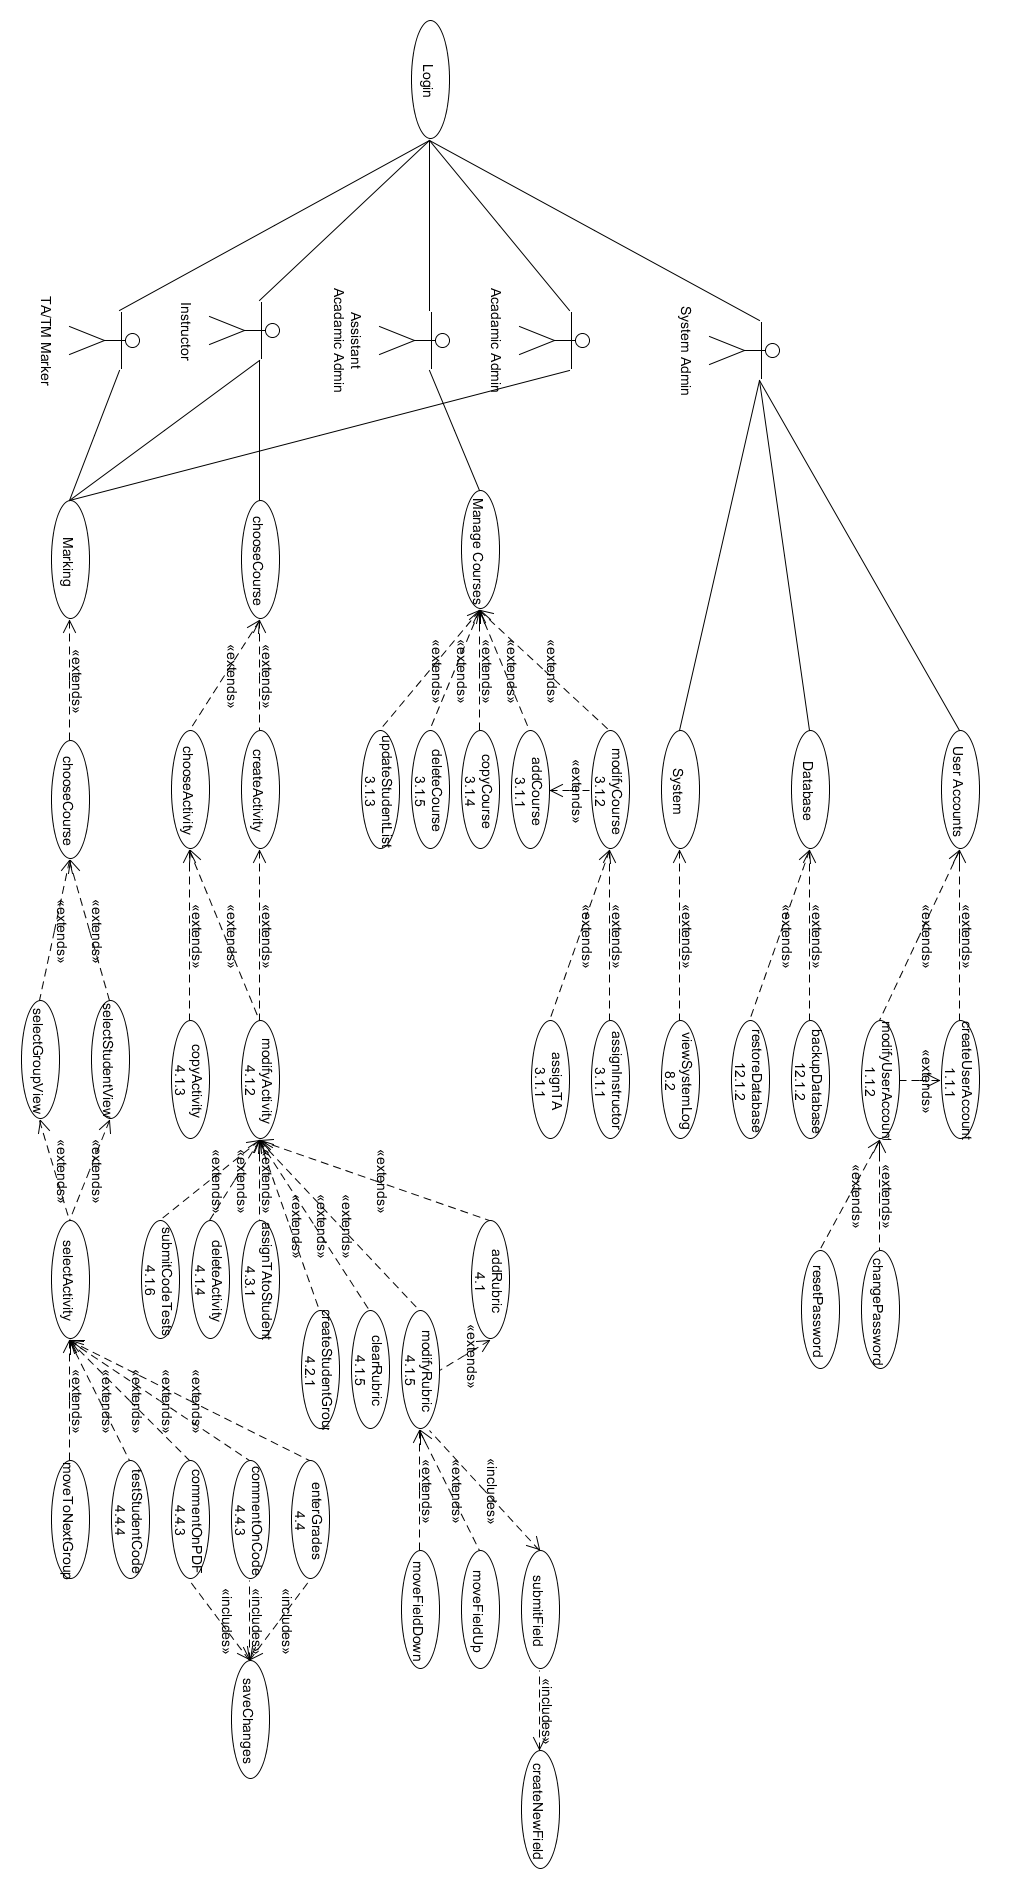
\includegraphics[scale=0.3]{../images/UseCaseDiagram}
\end{center}
\subsection{Descriptions}
\begin{itemize}
  \item createUserAccount \hfill \\
The System Admin clicks on the "Create Account" button. The fields are then filled in 
and the System Admin clicks confirm. The system stores the account info and returns to the userAccounts page
  \item modifyUserAccount \hfill \\
The System Admin clicks "Modify Account" button and selects the account to modify from a list. The System Admin 
then modifies the required fields and confirms. Password changes/resets are also handled here.
  \item changePassword \hfill \\
The System Admin goes to the modifyAccount page and clicks "Change Password". The System Admin then changes 
the password and confirms. The system resets the password and shows a confirmation.
  \item resetPassword \hfill \\
The System Admin goes to the modifyAccount page and clicks "Reset Password". The system asks for a second confirmation 
and generates a new password after the confirmation. The System Admin then sends the new password to the user.
  \item viewSystemLog \hfill \\
The System Admin selects this option and chooses the log s/he wishes to see.
  \item backupDatabase \hfill \\
The System Admin clicks the "Back Up Now" button, and a backup of the system is created. It is saved in a backup archive for up to 5 years.
  \item restoreDatabase \hfill \\
The System Admin clicks the "Restore Database" button. S/he then selects the backup to restore to and clicks "Restore". The system 
si reverted to that backup.

\item assignInstructor \hfill \\
The Assistant Academic Administrator will assign an instructor to a course.  The instructor will then have proper permissions for the course.
\item assignTA \hfill \\
The Assistant Academic Administrator will assign a TA/TM to a course.  The TA/TM will then have proper permissions for the course.
\item addCourse \hfill \\
The Assistant Academic Administrator will add course offerings.
\item modifyCourse \hfill \\
The Assistant Academic Administrator can modify a course offering.
\item copyCourse \hfill \\
The Assistant Academic Administrator can copy a previous course offering.  A course can be copied from a previous offering of the course (within 5 years).
\item deleteCourse \hfill \\
The Assistant Academic Administrator can delete a course offering.  A course cannot be deleted once an activity has be created.
updateStudentList \hfill \\
The Assistant Academic Administrator will update the student list for a course.  The student list will be a CSV.

\item createStudentGroup \hfill \\
This allows the Instructor to create groups of students to be graded together for a specific activity or set of activities satisfying requirement 4.2.1. The groups can then be marked as a whole, but students can also be given individual grades.
\item assignTAtoStudent \hfill \\
This allows the Instructor to assign TAs to mark a subset of students in the class satisfying requirement 4.3.1. The TA can be assigned to any subset of groups or students in the class. These assignments can be for a specific activity or an entire course, and the TA can then only mark sets assigned to them.
\item createActivity \hfill \\
This seems to be the main use case you did above.
\item modifyActivity \hfill \\
The instructor can modify any existing detail of an activity, satisfying requirement 4.1.2. Any detail of a specific activity can be modified.
\item copyActivity \hfill \\
The instructor can copy an activity from a previous offering of a course, satisfying requirement 4.1.3. An activity can be copied from a previous offering of the course or any of the instructor’s previous courses (within 5 years). All the portions of the activity not specific to an offering will be copied.
\item deleteActivity \hfill \\
The instructor can delete an activity from the course, satisfying requirement 4.1.4. The activity will be removed from the database. Any details of the activity or grading done on it will be completely removed.
\item addRubric \hfill \\
The instructor will add a rubric they create when creating the activity, satisfying another portion of requirement 4.1.1. The rubric will include descriptions of grading sections, possible grades for that section, and the grade given to the student for that section.
\item modifyRubric \hfill \\
The instructor can modify a rubric, satisfying requirement 4.1.5. Any parts of the rubric can be changed, deleted, or new parts can be added. If a rubric is modified, the any grading for that activity must be redone.
\item clearRubric \hfill \\
The instructor can clear a rubric while modifying it, as a portion of requirement 4.1.5. If a rubric is cleared, then a new rubric must be added (or edited in) before any grading can be done on the assignment.
\item submitCodeTests \hfill \\
The instructor can add tests for a coding assignment, satisfying requirement 4.1.6. The tests will include inputs for the student's code and a solution against which the student's result will be compared. These tests will be used in the testing suite for grading coding activities.

  \item chooseCourse
The Marker will select a course to grade assignments on from a list of courses they are affiliated with.
  \item selectStudentView
The Marker selects "Student View" for assignment grading
  \item selectGroupView
The Marker selects "Group View" for assignment grading.
  \item selectActivity
The Marker selects the activity to mark
\item enterGrades \hfill \\
The TA/TM will enter grades for an assignment.  Grades will be typed into a field in the rubric.
\item commentOnCode \hfill \\
The TA/TM will comment on coding assignments.  Comments will be injected directly into the code.
\item commentOnPDF \hfill \\
The TA/TM will comment on PDF-formatted assignments.  Comments will be applied directly into the PDF.
\item saveChanges \hfill \\
The TA/TM will be able to save changes.  After adding grades or comments, there will be a button to save changes, instead of discarding them upon exit.
\item testStudentCode \hfill \\
The TA/TM will test coding assignments.  Input files and their correct/expected output will have been added during assignment creation.  The source code will be compiled and run the provided test cases.  The experimental console output will be compared with the theoretical output.
\item moveToNextGroup \hfill \\
The TA/TM can directly move from marking one group to the next.  This button does not automatically save changes.
\end{itemize}

\subsubsection{Create Activity}
\textbf{Functional Requirement:} \ref{CreateAct} \\
\textbf{Primary Actors:} Instructor \\
\textbf{Secondary Actors:} Database \\
\textbf{Preconditions:}
\begin{itemize}
	\item The instructor is a valid user, and is logged in.
	\item The course the instructor is adding an activity to exists.
	\item The instructor teaches the course the activity is being added to.
	\item The system is at its initial screen after login.
\end{itemize}
\textbf{Main Flow of Events:}
\begin{enumerate}
	\item The use case starts when the instructor selects the "Activity Management" tab.
	\item The instructor then chooses to "Add An Activity" which sends them to a page listing
		the courses they are currently the instructor of.
	\item The instructor then selects the desired course to add an activity to, and is sent to 	
		a page containing fields to enter all the necessary details of an activity.
	\item The instructor inputs the necessary details to create an activity into the fields for
		them:
	\begin{enumerate}
		\item Name of activity
		\item Activity description
		\item Type of activity
		\item Language of activity
		\item Group or individual activity
		\item Solution
		\item Rubric
		\begin{enumerate}
			\item 	Instructor presses the "Add Rubric" button.
			\item The instructor enters the description of the aspect being graded, and the 
					possible grade for that aspect.
			\item The above process (ii.) is repeated for as many rubric aspects as desired
					(possibly none).
			\item The instructor presses "Confirm" and the rubric is added to the activity.
					A message is displayed confirming the rubric has been added successfully.
			\item The instructor is returned to the form for details of the activity.
		\end{enumerate}
		\item Due date with penalties/bonuses
			\begin{enumerate}
				\item The instructor enters a due date for the submission.
				\item The instructor presses the "Bonuses/Penalties" button.
				\item The instructor enters hour cutoffs for bonuses or penalties along with
						percentages of bonus or penalty at the hour marks specified.
				\item The instructor presses "Confirm" and the bonuses and penalties are
						saved based on the due date specified. A message is displayed
						confirming the bonuses and penalties have been saved.
				\item The instructor is returned to the normal form for details of activities.
			\end{enumerate}
		\item Test input and output files (for coding activities only)
			\begin{enumerate}
				\item The instructor presses "Add Tests".
				\item The instructor is prompted to enter the locations of any testing input
						files, as well as the locations of solution output files for a specific
						input. 
				\item The instructor presses "Confirm" and the testing files' locations are
						registered in the database to be used for marking. A message is
						displayed confirming the tests have been saved.
				\item The instructor is returned to the normal form for details of activites.
			\end{enumerate}
	\end{enumerate}
	\item The instructor presses the "Confirm" button.
	\item The system verifies that the details entered for the activity are valid in every field.
	\item A message is displayed confirming that the activity details were correct and the
			activity has been added to the course.
	\item The system returns the user to their initial screen.
	\item The use case terminates once the instructor has been returned to the initial
			screen.
\end{enumerate}
\textbf{Postconditions:}
\begin{itemize}
	\item The system has saved the activity in the database in the proper course.
	\item The system has returned to the instructor's initial screen.
\end{itemize}
\textbf{Exceptional Flow of Events:}
\begin{enumerate}
	\item \underline{Details for activity are not complete:} If the instructor did not specify
			all the necessary details for creating an activity, a message will be displayed
			stating which fields were empty when the instructor attempted to confirm.
			They will remain on the form for the activity, and be prompted to fill in necessary
			fields.
	\item \underline{Invalid data for a field of the activity:} If the instructor enters invalid
			data for one of the details of the assignment, a message will be displayed
			specifying which field contained invalid data. They will remain on the form and
			be prompted to correct errors in their entries.
\end{enumerate}

% Shorter 2nd Use Case description here.

\subsubsection{Summary Use Case: Marking an Activity}

% \textbf{Functional Requirement} \ref{}

\textbf{Primary Actors:} Instructors, TA/TM Markers \\
\textbf{Secondary Actors:} Database \\
\textbf{Preconditions:}
\begin{itemize}
\item Network is running.
\item Marker is a valid marker and logged in.
\item Initial welcome screen displayed containing options available to Marker.
\item The assignment, rubric and course exist
\item User is marking an assignment they are associated with
\item Database is functional
\end {itemize}

\textbf{Main Flow of Events:}
\begin{enumerate}
\item The use case starts when the Marker selects the Marking tab
\item The marker selects a course from the selection they are provided, which then redirects them to a new page for a list of assignments available.
\item The marker selects the assignment they want to mark on which is organized by submission of group/student. 
\item The marker views the assignment, and enters the following data:
	\begin {enumerate}
	\item “Grade”
		\begin {enumerate}
			\item  The user inputs the grade directly into the appropriate section of the rubric.
		\end {enumerate}
	\end {enumerate}
\item The Marker clicks the ‘Save’ button to update the database with the changes they have just made.
\item The system checks that the input data is in correct format (a number greater than or equal to 0).
\item A message is displayed stating that the mark has been successfully added.
The use case terminates after the message has been closed by the “OK” button.
\end {enumerate}

\textbf{Postconditions:}
\begin{itemize}
\item System saves the mark to the database
\item System returns to the marker’s initial screen
\end {itemize}

\textbf{Exceptional Flow of Events:}
\begin{enumerate}

\item \underline {Invalid mark entered:} If the marker enters non-conformable values for the mark (a mark that is less than 0 or empty) and presses save then:
	\begin {itemize}
		\item The system displays a message stating the mistake.
		\item The marker correct their mistake
		\item The marker selects “save”
		\item The use case continues in the normal fashion starting from step 6.
	\end {itemize}
\item \underline {No submission found:}
If the marker clicks onto an assignment that has not been submitted, then the system displays a message stating the mistake and returns the user back to the same page after closing the message tab.

\item \underline {Changes not saved:} If the marker has made changes but clicks ‘back’ or’’next’ without clicking ‘save’, the user will be offered a prompt asking if they would like to save their changes or move on without saving.
\item \underline {If no more submissions are available :} If the marker clicks ‘next’ and there is no further submissions available to mark, then:
\begin {itemize}
	\item The system displays a message stating the situation.
	\item The system takes the user back to the assignment selection page, ready for any further modifications
	\item The user can continue to select any assignment for remarking or can leave the page by pressing “back”
\end {itemize}

\item \underline {Lost connection:} If the marker’s client program loses connection to the database, then: 
\begin {itemize}
\item The system displays a message stating the connection is lost. 
\item The system takes the user back to the login page.
\end {itemize}
\end {enumerate}

\section{Class Diagram}
\begin{center}
  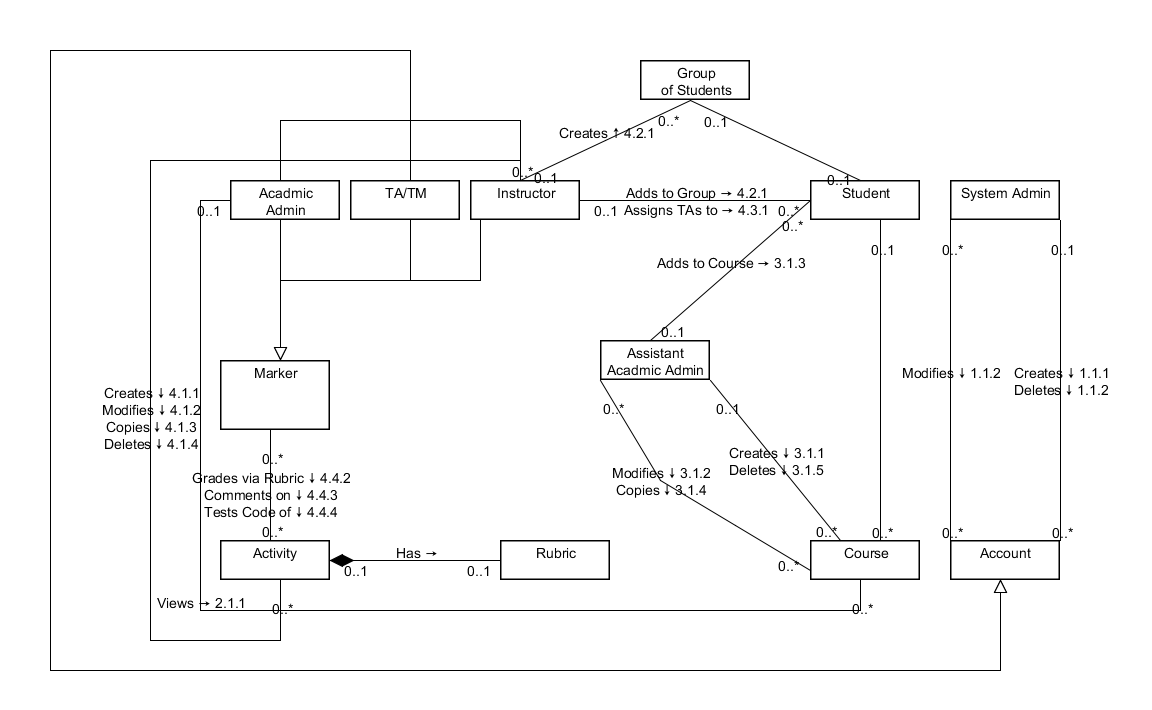
\includegraphics[scale=0.6]{../images/ClassDiagram}
\end{center}

\section{Scenarios}
\subsection{Grade and Save Changes}
Instructor Lee logs in, navigates to his Marking tab, then selects the course MATH 151.
He selects the student Mary’s submission for Homework 3, which was a series of multiple
choice math questions. He checks Mary’s submitted answers side-by-side with the solutions.
There were 20 questions worth 1 point each and Mary had 18 correct, so Instructor
Lee enters 18 into the points received portion of the rubric. He then clicks Save to update
the database, and it saves successfully.

\subsection{Grade and Discard Changes}
TA Jane logs in, navigates to her marking tab, then selects the course PHIL 100. She
selects the student Bill’s submission for Essay 2. The pdf of the essay is opened and
its rubric is shown beside it. Halfway through marking the essay and having already
filled in the marks for half of the rubric’s criteria, Jane realizes she had been repeatedly
misreading some key words and it changed the meaning of most of the essay. She decides
to regrade the entire essay, so she clicks on Discard Changes. A dialogue window pops
up that asks “You are going to discard changes. All unsaved changes will be lost. Are you
sure you want to continue?” with the options yes and no. She chooses yes and all the
changes she made to the rubric were reset. She now still has the same view, but the
rubric is back to its initial state with no marks entered.

\subsection{Comment on Code and Save Changes}
Instructor Lee logs in, navigates to his Marking tab, then selects the course CMPT 120.
He selects the student Ned’s submission for Code Assignment 4, which is a short Java
program. The code submission is presented in a text-editable box and the rubric is shown
beside it. As he is marking, Instructor Lee notices some portions of the code could have
been written more efficiently, so he enters a Java comment directly into the code which
suggests a possible improvement. He clicks Save which saves all the marks he had input
into the rubric, and also saves the updated code with his comments. A copy of the student’s
original submission still exists, but there is now also a copy which includes Instructor Lee’s
comments. Instructor Lee’s view is now still of the commented submission and the rubric with
the marks that have already been entered.


\end{document}
% Nothing past this will be included in the document.
